\documentclass[fontset=windows]{article}
\usepackage[margin=1in]{geometry}
\usepackage{ctex}
\usepackage{setspace}
\usepackage{lipsum}
\usepackage{graphicx}
\usepackage{caption}
\usepackage{subcaption}
\usepackage[colorlinks=true,linkcolor=red]{hyperref}
\usepackage{amsmath}
\usepackage{lmodern}

\graphicspath{{figures/}}

\title{\heiti\zihao{2} Source Followers \& Summary}
\author{\songti zrrraa}
\date{2023.12.19}

\begin{document}
\maketitle
\thispagestyle{empty}

\section*{Source Followers}

\begin{figure}[htbp]
    \centering
    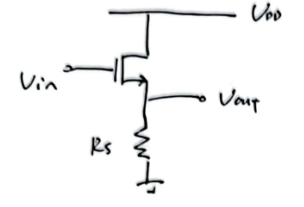
\includegraphics[scale=0.8]{1.jpg}
    \captionsetup{labelformat=empty}
    \caption{}
    \label{1}
\end{figure}

Draw the small signal model. 

\begin{figure}[htbp]
    \centering
    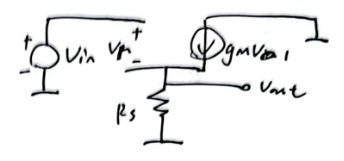
\includegraphics[scale=0.8]{2.jpg}
    \captionsetup{labelformat=empty}
    \caption{}
    \label{2}
\end{figure}

We get: 

\begin{equation*}
    \begin{cases}
        v_{in}=v_1+v_{out} \\
        \frac{v_{out}}{R_s}=g_mv_1
    \end{cases}
\end{equation*}

So: 

$$A_v=\frac{R_s}{\frac{1}{g_m}+R_s}$$

In other words, $A_v=\frac{Resistance\ tied\ between\ S\ and\ GND}{\frac{1}{g_m}+Resistance\ tied\ between\ S\ and\ GND}$. 

\section*{Alternative Analysis}

We can also use Thevenin Equivalent to analyze the source follower. 

First, let's think of the source follower as a voltage source. 

\begin{figure}[htbp]
    \centering
    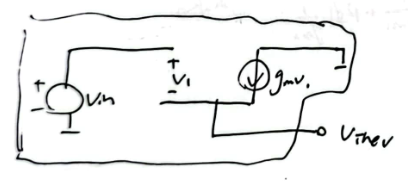
\includegraphics[scale=0.8]{3.jpg}
    \captionsetup{labelformat=empty}
    \caption{}
    \label{3}
\end{figure}

$$g_mv_1=0\Longrightarrow v_1=0\Longrightarrow v_{in}=v_{Thevenin}$$

Then let's kill the independent voltage source. 

\begin{figure}[htbp]
    \centering
    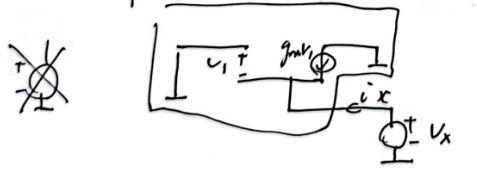
\includegraphics[scale=0.8]{4.jpg}
    \captionsetup{labelformat=empty}
    \caption{}
    \label{4}
\end{figure}

\begin{equation*}
    \begin{cases}
        i_x=-g_mv_1 \\
        v_1=-v_x
    \end{cases}
\end{equation*}

$$\Longrightarrow R_x=\frac{v_x}{i_x}=\frac{-v_1}{-g_mv_1}=\frac{1}{g_m}$$

So we can get the simple model: 

\begin{figure}[htbp]
    \centering
    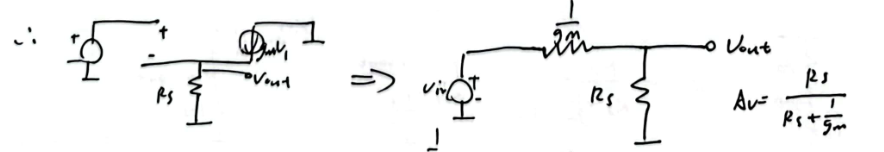
\includegraphics[scale=0.8]{5.jpg}
    \captionsetup{labelformat=empty}
    \caption{}
    \label{5}
\end{figure}

$$A_v=\frac{R_s}{R_s+\frac{1}{g_m}}$$

The same as we derive just now. 

If $\lambda \neq 0$: 

\begin{figure}[htbp]
    \centering
    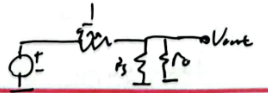
\includegraphics[scale=0.8]{6.jpg}
    \captionsetup{labelformat=empty}
    \caption{}
    \label{6}
\end{figure}

$$A_v=\frac{R_s||r_o}{R_s||r_o+\frac{1}{g_m}}$$

$$R_{out}=\frac{1}{g_m}||R_s||r_o$$

\section*{Application of Source Follower}

If we want to radiate the amplified signal through the antenna, we can use a CS Stage. 

\begin{figure}[htbp]
    \centering
    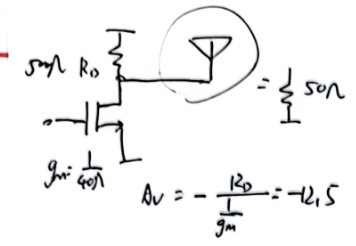
\includegraphics[scale=0.8]{7.jpg}
    \captionsetup{labelformat=empty}
    \caption{}
    \label{7}
\end{figure}

For the CS Stage, $$A_v=-\frac{R_D}{\frac{1}{g_m}}=12.5$$. 

The resistance of antenna is usually very small, such as, $50\Omega$. 
The gain decrease a lot because of this. 

$$A_v=-\frac{R_D||R_{ant}}{\frac{1}{g_m}}=-1.14$$

In this way we can use a source follower. 

\begin{figure}[htbp]
    \centering
    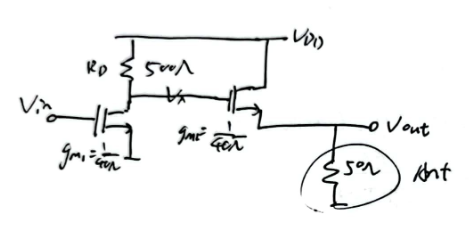
\includegraphics[scale=0.8]{8.jpg}
    \captionsetup{labelformat=empty}
    \caption{}
    \label{8}
\end{figure}

$$A_v=\frac{v_{out}}{v_{in}}=\frac{v_x}{v_{in}\frac{v_{out}}{v_x}}=-g_{m1}R_D*\frac{R_s}{\frac{1}{g_{m2}}+R_s}=-6.9$$

Source follower suppresses gain reduction. 

\section*{Example}

\begin{figure}[htbp]
    \centering
    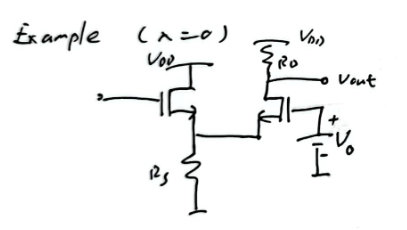
\includegraphics[scale=0.8]{9.jpg}
    \captionsetup{labelformat=empty}
    \caption{}
    \label{9}
\end{figure}

$$A_v=\frac{R_s||\frac{1}{g_{m1}}}{\frac{1}{g_{m1}}+R_s||\frac{1}{g_{m2}}}*g_{m2}R_D$$

\section*{Bias Design}

\begin{figure}[htbp]
    \centering
    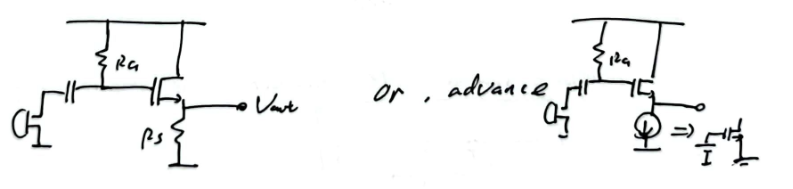
\includegraphics[scale=0.8]{10.jpg}
    \captionsetup{labelformat=empty}
    \caption{}
    \label{10}
\end{figure}

We can create bias by adding a resistor between gate and $V_{DD}$. 

In order to reduce the loss of gain caused by the source follower, a current source can be used instead of the source resistor. 

\section*{Summary}

The three structures show different situations when the input and output are at the source, drain and gate of the MOSFET respectively. 

For $\lambda =0$

\begin{figure}[htbp]
    \centering
    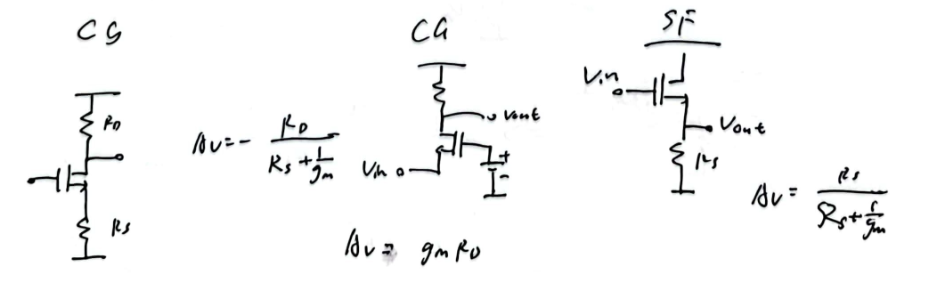
\includegraphics[scale=0.9]{11.jpg}
    \captionsetup{labelformat=empty}
    \caption{}
    \label{11}
\end{figure}

\subsection*{CS Stage}

$$A_v=-\frac{R_D}{R_s+\frac{1}{g_m}}$$

\subsection*{CG Stage}

$$A_v=g_mR_D$$

\subsection*{SF}

$$A_v=\frac{R_s}{R_s+\frac{1}{g_m}}$$

\section*{Link}

\href{https://www.bilibili.com/video/BV1FD4y1R7Ah?p=41&vd_source=1d0c07486a3bd3b0adb8ac548bf6453e}{Razavi Electronics Circuits 1: lectrue 41}
\end{document}